\begin{figure}[p]
\centering
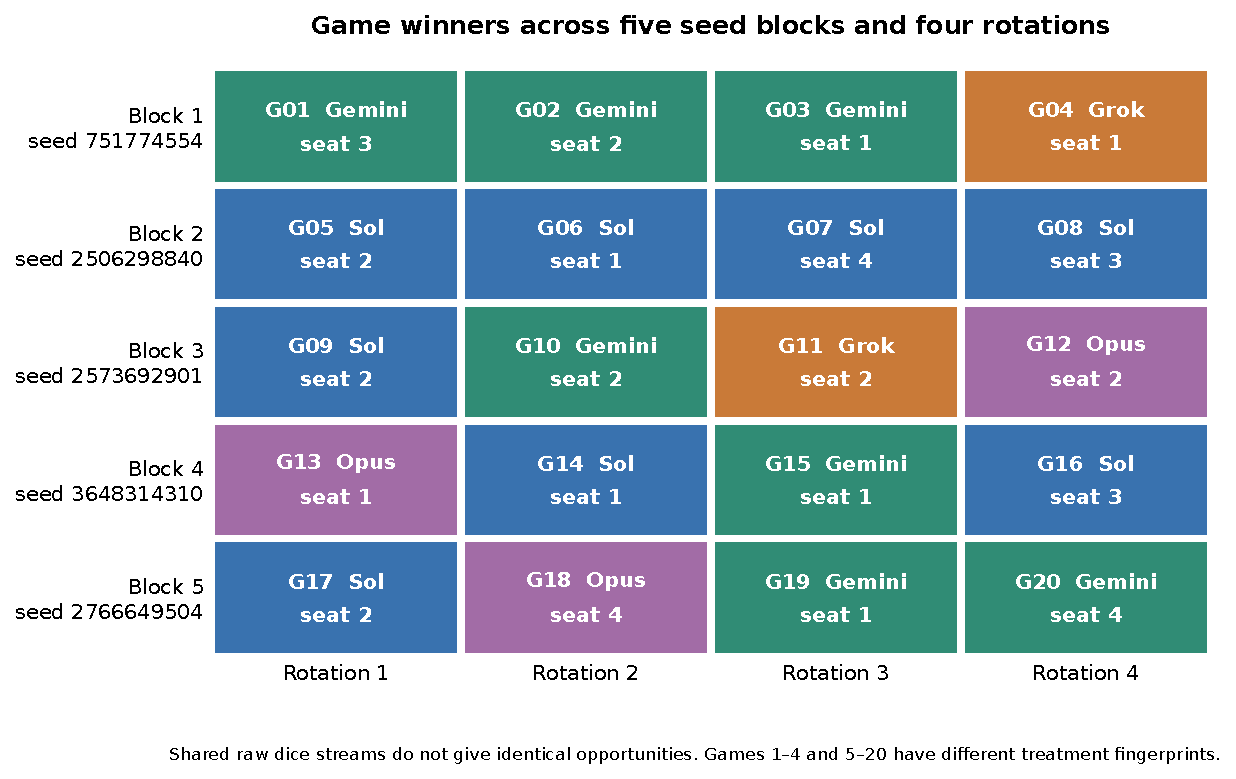
\includegraphics[width=\linewidth,height=0.57\textheight,keepaspectratio]{f02_seed_rotation_winners.pdf}
\caption[Outcomes across seed blocks and seat rotations]{Each cell is one complete game. All four models occupy each seat five times. Block 2 has the same model win across four seats; block 3 has the same seat win with four models. Neither pattern identifies a pure skill or luck component. Raw dice prefixes are shared within blocks, but draw use, subsequent positions, jail and eliminations differ. Games 1--4 and 5--20 have different saved treatment fingerprints. Seat numbers are \textbf{one-based p1--p4}, so the block-3 sweep is seat 2; older zero-based reports called it seat 1. Win counts describe this cohort, not an intrinsic ranking. Source: Sol's phase-2 design reconstruction, independently checked against the Astra economics audit.

F2 source-version note: the 18-file commit diff changes campaign-concurrency plumbing, UI/API, documentation and tests; no engine, prompt, resolver, player-configuration or model-client file changes. Neither a behavioral effect nor its absence is inferred from the diff. The refusal-share shift coincides with this boundary without an identified cause. Underlying data: Table~\ref{tab:t01_cohort}.}
\label{fig:f02_seed_rotation_winners}
\end{figure}
